\section{Common Language Infrastructure}
\label{sec:cts}
The entire CLI has been documented, standardized and approved~\cite{Ecma-335} by the European association for standardizing information and communication systems, Ecma International\footnote{An European industry association founded in 1961 and dedicated to the standardization of Information and Communication Technology (ICT) Systems.
Their website can be found at \url{http://www.ecma-international.org/}.}.
Benefits of this CLI for developers and end-users are:

\begin{itemize}[noitemsep]
  \item Most high level programming languages can easily be mapped onto the Common Type System (CTS);
  \item The same application will run on different CLI implementations;
  \item Cross-programming language integration, if the code strictly conforms to the Common Language Specification (CLS);
  \item Different CLI implementations can communicate with each other, providing applications with easy cross-platform communication means.
\end{itemize}

This interoperability and portability is, for instance, achieved by using a standardized meta data and intermediate language (CIL) scheme as the storage and distribution format for applications.
In other words, (almost) any programming language can be mapped to CIL, which in turn can be mapped to any native machine language.

The Common Language Specification is a subset of the Common Type System, and defines the basic set of language features that all \dotNET languages should adhere to.
In this way, the CLS helps to enhance and ensure language interoperability by defining a set of features that are available in a wide variety of languages.
The CLS was designed to include all the language constructs that are commonly needed by developers 
(\eg naming conventions, common primitive types), but no more than most languages are able to support~\cite{Microsoft03-2}.
\autoref{fig:Common_Type_System} shows the relationships between the CTS, the CLS, and the types available in C++ and C\#.
\begin{figure}[htbp]
 \centering
 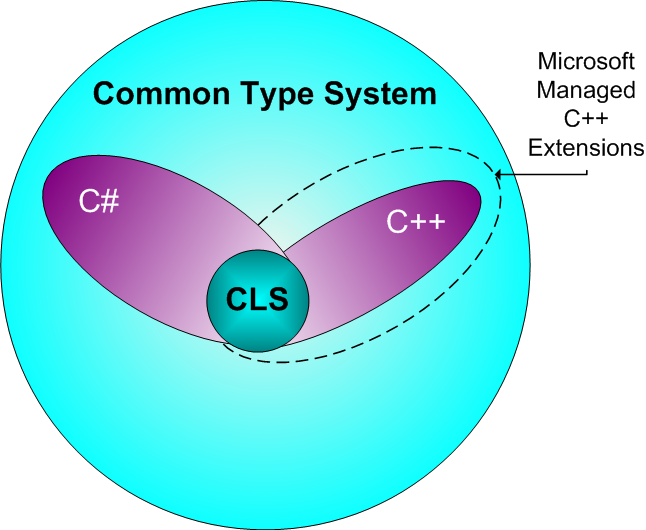
\includegraphics[style=fourthheight]{Common_Type_System}
 \caption{Relationships in the CTS}
 \label{fig:Common_Type_System}
\end{figure}
In this way the standardized CLI provides, in theory\footnote{Unfortunately Microsoft did not submit all the framework classes for approval and at the time of writing only the \dotNET Framework implementation is stable.}, a true cross-language and cross-platform development and runtime environment.

To attract a large number of developers for the \dotNET Framework, Microsoft has released CIL compilers for C++, C\#, J\#, and VB.NET.
In addition, third-party vendors and open-source projects also released compilers targeting the \dotNET Framework, such as Delphi.NET, Perl.NET, IronPython, and Eiffel.NET.
These programming languages cover a wide-range of different programming paradigms, such as classic imperative, object-oriented, scripting, and declarative languages. This wide coverage demonstrates the power of the standardized CLI.

\begin{figure}[htbp]
 \centering
 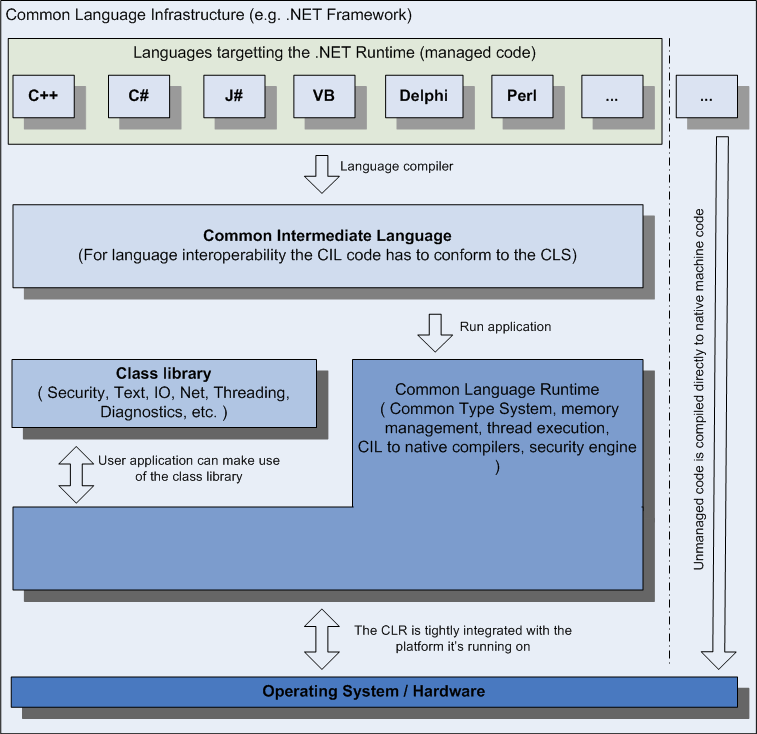
\includegraphics[style=halfheight]{Common_Language_Infrastructure}
 \caption[Main components of the CLI and their relationships]{%
    Main components of the CLI and their relationships.
    The right hand side of the figure shows the difference between managed code and unmanaged code.}
 \label{fig:Common_Language_Infrastructure}
\end{figure}

\autoref{fig:Common_Language_Infrastructure} shows the relationships between all the main components of the CLI.
The top of the figure shows the different programming languages with compiler support for the CLI. Because the compiled code is stored and distributed in the Common Intermediate Language format, the code can run on any CLR. For cross-language usage this code has to comply with the CLS.
Any application can use the class library (the FCL) for common and specialized programming tasks. 